% !TEX TS-program = pdflatex
% !TEX encoding = UTF-8 Unicode

% This is a simple template for a LaTeX document using the "article" class.
% See "book", "report", "letter" for other types of document.

\documentclass[11pt]{article} % use larger type; default would be 10pt

\usepackage[utf8]{inputenc} % set input encoding (not needed with XeLaTeX)


%%% Examples of Article customizations
% These packages are optional, depending whether you want the features they provide.
% See the LaTeX Companion or other references for full information.

%%% PAGE DIMENSIONS
\usepackage{geometry} % to change the page dimensions
\geometry{a4paper} % or letterpaper (US) or a5paper or....
% \geometry{margin=2in} % for example, change the margins to 2 inches all round
% \geometry{landscape} % set up the page for landscape
%   read geometry.pdf for detailed page layout information
\usepackage{sidecap}
\usepackage{graphicx} % support the \includegraphics command and options

% \usepackage[parfill]{parskip} % Activate to begin paragraphs with an empty line rather than an indent

%%% PACKAGES
\usepackage{booktabs} % for much better looking tables
\usepackage{array} % for better arrays (eg matrices) in maths
\usepackage{paralist} % very flexible & customisable lists (eg. enumerate/itemize, etc.)
\usepackage{verbatim} % adds environment for commenting out blocks of text & for better verbatim
\usepackage{subfig} % make it possible to include more than one captioned figure/table in a single float
% These packages are all incorporated in the memoir class to one degree or another...

%%% HEADERS & FOOTERS
\usepackage{fancyhdr} % This should be set AFTER setting up the page geometry
\pagestyle{fancy} % options: empty , plain , fancy
\renewcommand{\headrulewidth}{0pt} % customise the layout...
\lhead{}\chead{}\rhead{}
\lfoot{}\cfoot{\thepage}\rfoot{}

\usepackage{amssymb}

%%% SECTION TITLE APPEARANCE
\usepackage{sectsty}
\allsectionsfont{\sffamily\mdseries\upshape} % (See the fntguide.pdf for font help)
% (This matches ConTeXt defaults)

%%% ToC (table of contents) APPEARANCE
\usepackage[nottoc,notlof,notlot]{tocbibind} % Put the bibliography in the ToC
\usepackage[titles,subfigure]{tocloft} % Alter the style of the Table of Contents
\renewcommand{\cftsecfont}{\rmfamily\mdseries\upshape}
\renewcommand{\cftsecpagefont}{\rmfamily\mdseries\upshape} % No bold!

%%% END Article customizations

%%% Theorem Environment
\newtheorem{theorem}{Theorem}[section]
\newtheorem{lemma}[theorem]{Lemma}
\newtheorem{proposition}[theorem]{Proposition}
\newtheorem{corollary}[theorem]{Corollary}

\newenvironment{proof}[1][Proof]{\begin{trivlist}
\item[\hskip \labelsep {\bfseries #1}]}{\end{trivlist}}
\newenvironment{definition}[1][Definition]{\begin{trivlist}
\item[\hskip \labelsep {\bfseries #1}]}{\end{trivlist}}
\newenvironment{example}[1][Example]{\begin{trivlist}
\item[\hskip \labelsep {\bfseries #1}]}{\end{trivlist}}
\newenvironment{remark}[1][Remark]{\begin{trivlist}
\item[\hskip \labelsep {\bfseries #1}]}{\end{trivlist}}
\newenvironment{assignment}[1][Assignment]{\begin{trivlist}
\item[\hskip \labelsep {\bfseries #1}]}{\end{trivlist}}

\newcommand{\qed}{\nobreak \ifvmode \relax \else
      \ifdim\lastskip<1.5em \hskip-\lastskip
      \hskip1.5em plus0em minus0.5em \fi \nobreak
      \vrule height0.75em width0.5em depth0.25em\fi}

\usepackage{listings}
\usepackage{color}

\definecolor{dkgreen}{rgb}{0,0.6,0}
\definecolor{gray}{rgb}{0.5,0.5,0.5}
\definecolor{mauve}{rgb}{0.58,0,0.82}

\lstset{frame=tb,
  language=Java,
  aboveskip=3mm,
  belowskip=3mm,
  showstringspaces=false,
  columns=flexible,
  basicstyle={\small\ttfamily},
  numbers=none,
  numberstyle=\tiny\color{gray},
  keywordstyle=\color{blue},
  commentstyle=\color{dkgreen},
  stringstyle=\color{mauve},
  breaklines=true,
  breakatwhitespace=true,
  tabsize=3
}



%%% END Theorem Environment

%%% The "real" document content comes below...


\title{Exponential Distribution Simulation}
\author{Michael Lee}
\date{August 21, 2015} % Activate to display a given date or no date (if empty) % otherwise the current date is printed 

\begin{document}
\maketitle

\section{Overview}
  The Central Limit Theorem states that the distribution of averages of independently and identically distributed variables becomes a standard normal distribution as the sample size gets larger. Here we will use randomized samples of the exponential distribution to demonstrate the CLT by comparing the theoretical mean to the sample mean and the theoretical variance to the sample variance.

\section{Simulation}
	The exponential distribution is a probability distribution function, parametrised by $\lambda$, whose theoretical mean and standard deviation $ = \frac{1}{\lambda}$. We want to show that as the sample size of the exponential distibution gets larger, the distribution of the averages of the exponential distribution approaches a normal distribution. To demonstrate this limiting behavior, we will generate a thousand averages from random exponential distributions with constant rate $\lambda = 0.2$ and sample size $n = 40$. We hold $\lambda$ and $n$ constant to satisfy the independently and identically distributed condition of the CLT.

\begin{lstlisting}
	n <- 1000 
	lambda <- 0.2 
	MNS <- NULL # average distribution
	for (i in 1 : 1000) MNS = c(MNS, mean(rexp(40,lambda)))  
	hist(MNS) 
\end{lstlisting}

\section{Mean}

The mean is a central tendency of a distribution, it represents the center of mass of a collection of locations and weights. There are two kinds of means: theoretical $(\mu)$ and sample $(\bar{x})$. The theoretical mean is calculated by integrating the expected value function and probability mass function. The sample mean is calculated by summing the arithmetic averages of empirical events.  

\subsection{Theoretical Mean}
	We know that the theoretical mean of an exponential distribution is $\mu = \frac{1}{\lambda} = \frac{1}{.2} = 5$. 
\subsection{Sample Mean}
	The Law of Large Numbers suggests that as the sample size increases, the sample mean approaches the theoretical mean. We would then expect that the sample mean of 1000 means of 40 random exponential distributions would be very close to the theoretical mean of $\mu = 5$.  The following R code computes the sample mean:
\begin{lstlisting}
	sampleMean <- mean(MNS)
	sampleMean
\end{lstlisting} 

\begin{lstlisting}
	5.014358
\end{lstlisting}
	As expected, $\bar{x} \approx \mu$. \\
To further illustrate this behavior, we plot the distribution of averages as a density plot and draw a vertical line over the sample mean. 

\begin{lstlisting}
	ggplot() + aes(MNS) + 
	geom_density() + 
	geom_vline(xintercept = sampleMean, size = 1, color = 'red')
\end{lstlisting}

\begin{SCfigure}
  \centering
\caption{\footnotesize Density Plot of 1000 averages of $n = 40, \lambda = 0.2$ random exponential distributions. The x-intercept of the redline is the sample mean which is very close to the mean of the original exponential disitribution $\mu = 5$. Note the concentration of density surrounding the sample mean.}
  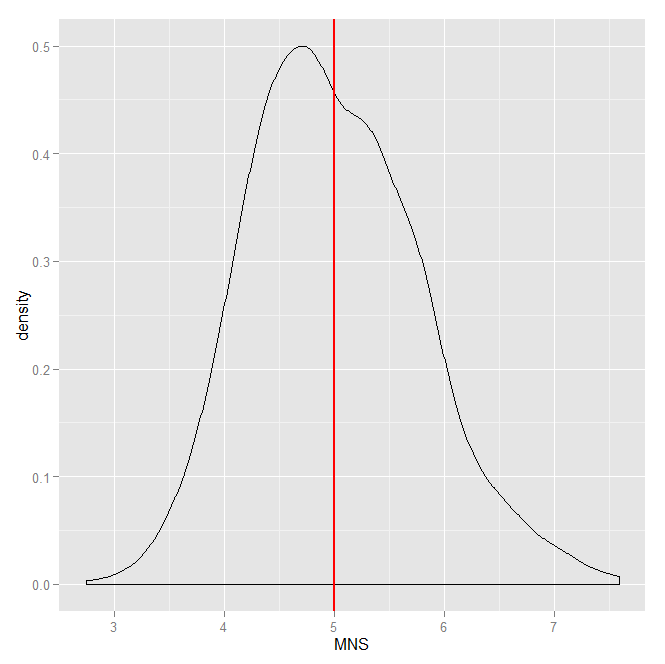
\includegraphics[scale = 0.45]{figure1}
	\label{Figure 1.}
\end{SCfigure}

\section{Variance}
	The variance of a random variable is a measure of its spread. Variance indicates the relative span and density of a set of numbers, i.e. a small variance implies a dense distribution around the mean over a short span and a large variance implies a sparse distribution around the mean over a large span.  Like the mean, there are two variances: theoretical ($\sigma^2$) and sample ($S^2$).The theoretical variance is the expected value of the squared distance the population and its theoretical mean. 
The sample variance is the summation of the unbiased average squared distance between the population and the sample mean. 
{\center
	$\sigma^2 = E[(X - \mu)^2] = \Sigma_{i = 1}^{n}{\frac{(X_i - \mu)^2}{n}} \mid S^2 = \Sigma_{i = 1}^{n}{\frac{(x_i - \bar{x})^2}{n - 1}}$
}
\subsection{Sample}
The following R code computes the variance of MNS and standard derivation:
	\begin{lstlisting}
		sampleVar <- var(MNS)
		std <- sd(MNS)
	\end{lstlisting}
	\begin{lstlisting}
		0.6021728
 		0.7759979
	\end{lstlisting}

\subsection{Theoretical}
	Since the sample variance is a function of the sample mean, it has an associated population distribution.
	{\center
		$ Var(\bar{X})  = Var(\frac{\Sigma_{i = 1}^{n}{X_i}}{n}) $ \\ 
		$ Var(\bar{X}) =  Var(\frac{X_1}{n} + \frac{X_2}{n} \ldots + \frac{X_n}{n}) $ \\ 
		$ Var(\bar{X}) = \frac{1}{n^2}(Var(X_1) + Var(X_2) + \ldots + Var(X_n)) $ \\ 
		Since the sample mean is identically distributed,$ Var(X_{1, 2, \ldots, n}) = \sigma^2 $\\ 
		$ Var(\bar{X}) = \frac{1}{n^2}(\sigma^2 + \sigma^2 + \ldots + \sigma^2) $ \\ 
		$ Var(\bar{X}) = \frac{1}{n^2}{n \cdot \sigma^2} = \frac{\sigma^2}{n}$ \\
		Recall that $\sigma = \frac{1}{\lambda} = 5$ \\ 
		$ Var(\bar{X}) = \frac{5^2}{40} = 0.625 $ \\ 
		$ std(\bar{X}) = sqrt(Var(\bar{X})) = 0.791 $ \\
	}
To further illustrate the spread, we plot the distribution of averages as a density plot and draw vertical lines over the sample mean and one standard deviation away from the sample mean. 

\begin{lstlisting}
	ggplot() + aes(MNS) + 
	geom_density() + 
	geom_vline(xintercept = sampleMean, size = 1, color = 'red') +
	geom_vline(xintercept = (sampleMean + std), size = 1, color = 'blue') +
	geom_vline(xintercept = (sampleMean - std), size = 1, color = 'blue')
\end{lstlisting}

\begin{SCfigure}
  \centering
\caption{\footnotesize Density Plot of 1000 averages of $n = 40, \lambda = 0.2$ random exponential distributions. The x-intercept of the redline is the sample mean. The x-intercepts of the blue lines are one standard deviation away from the mean. Compare the distance (i.e. spread) of one standard deviation to the domain of the plot.}
  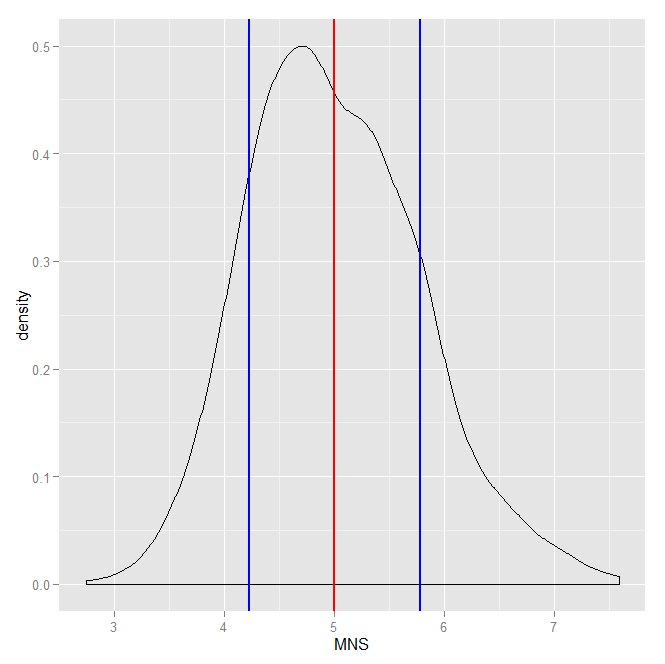
\includegraphics[scale = 0.45]{figure2}
	\label{Figure 2.}
\end{SCfigure}

\section{Normal Distribution}

\begin{theorem}
	$\mathbf{Central \> Limit \> Theorem.}$ The distribution of averages of independently and identically distributed variables approaches a standard normal distribution as the sample size increases. 
\end{theorem}
	The constants $\lambda = 0.2$ and $n = 40$ satisfy the condition of independently and identically distributed variables, but now we need to verify whether the distribution of averages $\cong$ standard normal. \\

To illustrate the normalcy of MNS, we plot MNS as a density plot as well as the non-standard normal distribution $Z \cong (\mu = \frac{1}{\lambda}, sd = \frac{sqrt(var(X))}{sqrt(n)})) $ \\
\begin{lstlisting}
mu    <- 1/lambda
sigma <- 1/lambda
ggplot() + aes(MNS) + 
geom_histogram(alpha = .10, binwidth=0.1, colour = "black", aes(y = ..density..)) +
stat_function(geom = "line", fun = dnorm, arg = list(mean = mu, sd = sigma/sqrt(40)), size = 1, colour = "green", fill = NA)
\end{lstlisting}
\end{document}

\begin{SCfigure}
  \centering
\caption{\footnotesize Density Plot of 1000 averages of $n = 40, \lambda = 0.2$ random exponential distributions. Trace of non-standard normal distribution $Z \approx (\mu = \frac{1}{\lambda}, sd = \frac{\sigma}{sqrt(n)})) $. The normal distribution's arguments are based on calculations made in sections 3 and 4.  }
  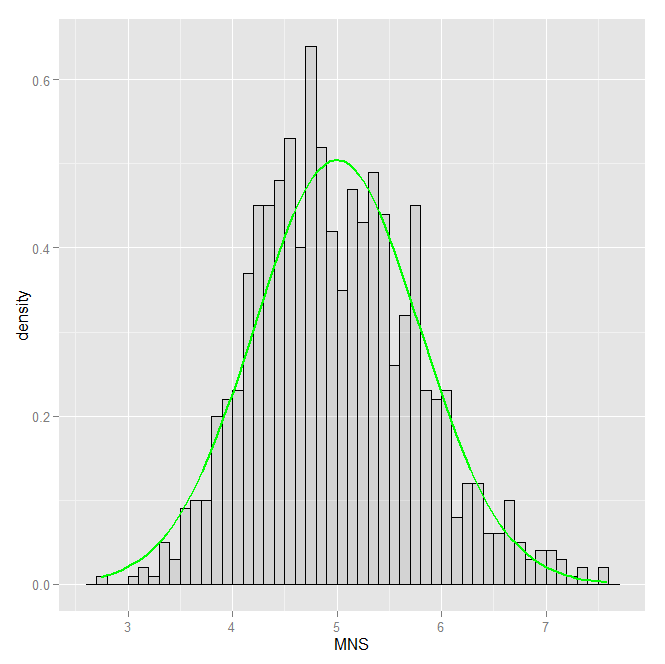
\includegraphics[scale = 0.45]{figure3}
	\label{Figure 3.}
\end{SCfigure}

